\section{Introduction}
Measuring environmental parameters in and around the water in Greenland (or any watery nation) is a time consuming task. Today measurements are carried out by manually navigating large vessels up and down along the coastline and into the fjords. 

The purposes of these measurements could be to measure the water depth for bathymetric surveys. This would allow for safer voyages in and around the coastlines, and for general environmental studies. 

These measurements are today carried out by one large vessel, which could be exchanged for several smaller ones to reduce the surveying time and labor cost. This would make for a faster measurement of the coastline as well as giving an opportunity to measure previously un-surveyed waters due to costs. 

Reducing the size of a vessel, poses some other challenges in regards to the weather conditions and other environmental parameters, that has a much larger influence on small scale vessels, than on larger ones. This paper will deal with how such a surveying vessel can be developed, and still measure the water depth whilst under the influence of the above.

A challenge using a single beam transducer to measure water depth is the roll/pitch of the craft. Figure \vref{fig:beamer} illustrates this problem, where an induced pitch of the ship (eg. a wave) makes it impossible for the vessel to make a precise measurement.

\begin{figure}[h]
\centering
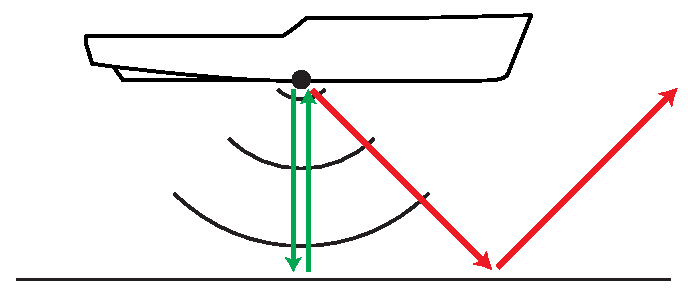
\includegraphics[width=0.5\textwidth]{img/beamer}
\caption{Overview of a depth mapping system. The green represents a measurement shot directly down and the red represents a measurement with induced pitch on the ship}
\label{fig:beamer}
\end{figure}

